\textbf{Aclaración}: La notación $C^k_n$ es lo mismo que $\binom{n}{k}$


\section{Triángulo de Pascal}

\subsection{Definición}

\begin{definicion}
    En las matemáticas, el \textbf{triángulo de Pascal} es una representación de los coeficientes binomiales ordenados en forma de triángulo. Es llamado así en honor al filósofo y matemático francés Blaise Pascal, quien introdujo esta notación en 1654, en su trabajo \textit{Traité du triangle arithmétique}.
\end{definicion}

Acomodemos en una tabla los valores de $C^{k}_{n}$ con los valores de $n$ por filas y los de $k$ por columnas:

\begin{center}
    \begin{tabular}{|cc|ccccccccc|}
    \hline
      & r & 0 & 1 & 2  & 3  & 4  & 5  & 6  & 7 & 8 \\
    n &   &   &   &    &    &    &    &    &   &   \\ \hline
    0 &   & 1 &   &    &    &    &    &    &   &   \\
    1 &   & 1 & 1 &    &    &    &    &    &   &   \\
    2 &   & 1 & 2 & 1  &    &    &    &    &   &   \\
    3 &   & 1 & 3 & 3  & 1  &    &    &    &   &   \\
    4 &   & 1 & 4 & 6  & 4  & 1  &    &    &   &   \\
    5 &   & 1 & 5 & 10 & 10 & 5  & 1  &    &   &   \\
    6 &   & 1 & 6 & 15 & 20 & 15 & 6  & 1  &   &   \\
    7 &   & 1 & 7 & 21 & 35 & 35 & 21 & 7  & 1 &   \\
    8 &   & 1 & 8 & 28 & 56 & 70 & 56 & 28 & 8 & 1 \\ \hline
    \end{tabular}
\end{center}

También pueden ubicarse en un arreglo simétrico de la siguiente manera:

\begin{center}
\begin{tabular}{p{0.6cm} p{0.6cm} p{0.6cm} p{0.6cm} p{0.6cm} p{0.6cm} p{0.6cm} p{0.6cm} p{0.6cm} p{0.6cm} p{0.6cm} p{0.6cm} p{0.6cm} p{0.6cm} p{0.6cm} p{0.6cm} p{0.6cm}}
  &   &   &   &    &    &    &    & \centering1  &    &    &    &    &   &   &   &   \\
  &   &   &   &    &    &    & \centering1  &    & \centering1  &    &    &    &   &   &   &   \\
  &   &   &   &    &    & \centering1  &    & \centering2  &    & \centering1  &    &    &   &   &   &   \\
  &   &   &   &    & \centering1  &    & \centering3  &    & \centering3  &    & \centering1  &    &   &   &   &   \\
  &   &   &   & \centering1  &    & \centering4  &    & \centering6  &    & \centering4  &    & \centering1  &   &   &   &   \\
  &   &   & \centering1 &    & \centering5  &    & \centering10 &    & \centering10 &    & \centering5  &    & \centering1 &   &   &   \\
  &   & \centering1 &   & \centering6  &    & \centering15 &    & \centering20 &    & \centering15 &    & \centering6  &   & \centering1 &   &   \\
  & \centering1 &   & \centering7 &    & \centering21 &    & \centering35 &    & \centering35 &    & \centering21 &    & \centering7 &   & \centering1 &   \\
\centering1 &   & \centering8 &   & \centering28 &    & \centering56 &    & \centering70 &    & \centering56 &    & \centering28 &   & \centering8 &   & \centering1
\end{tabular}
\end{center}

La \textbf{Identidad de Pascal} nos dice que todo elemento del triángulo es igual a la suma de los dos que se encuentran directamente sobre él. Esto quiere decir que si construimos un arreglo triangular de números (comenzando y terminando cada fila con 1), de modo que todo número interior sea la suma de los dos que están encima de él, los números que aparecen son precisamente los números combinatorios. 

El triángulo de Pascal encierra muchas relaciones numéricas, por ejemplo, la suma de todos los números en la n-ésima fila es $2^{n-1}$.

\section{Teorema del binomio}

\subsection{Problema introductorio}

Consideremos $(a+b)^5$. Al desarrollarlo, ¿con qué coeficiente aparece el término cuya parte literal es $a^3b^2$?

Para desarrollar $(a+b)^5= (a+b)(a+b)(a+b)(a+b)(a+b)$, de cada factor hay que seleccionar la $a$ o la $b$ y luego multiplicar esos cinco términos. Por ejemplo, el arreglo $aabba$ representa el escoger la $a$ en los factores primero, segundo y quinto, y escoger la $b$ en los factores tercero y cuarto. Como en cada factor hay dos opciones para elegir, la cantidad de posibles arreglos es $2^5= 32$, pero de estos arreglos algunos serán términos semejantes, por ejemplo $aabba$, $bbaaa$, $ababa$ y $baaab$ son algunos de los arreglos que corresponden al término $a^3b^2$, de manera que el coeficiente del término con parte literal $a^3b^2$ en el desarrollo de $(a+b)^5$ se obtiene al contar la cantidad de arreglos de cinco letras que pueden hacerse con tres $a$ y dos $b$, esto es $C^{3}_{5}$ porque solo se necesita seleccionar entre los 5 espacios disponibles los 3 que serán ocupados por las $a$ y luego las $b$ se colocan automáticamente, como una cadena binaria.

Ahora, si estudiamos el caso general, al desarrollar $(x+y)^n$, como son $n$ factores, cada arreglo estará formado por $n$ letras de las cuales algunas, digamos $k$ (con $0 \leq k \leq n$), serán $y$ y el resto, $n-k$, serán $x$, por lo que el término con parte literal $x^{n-k} y^k$ tendrá coeficiente $C^{k}_{n}$. Además, como hay $n+1$ opciones para los valores de $k$ (es decir para la cantidad de $y$’s en el arreglo), el desarrollo de $(x+y)^n$ tendrá $n+1$ términos. 

\subsection{Teorema del binomio}

En general, el desarrollo del binomio $(x+y)^n$ es:

\begin{center}
    $(x+y)^n= C^{0}_{n} x^{n} + C^{1}_{n} x^{n-1} y^{1} + C^{2}_{n} x^{n-2} y^{2} + ... + C^{n-1}_{n} x^{1} y^{n-1} + C^{n}_{n} y^{n}$ \\ \hfill \\
    $(x+y)^n= \displaystyle\sum_{k=0}^{n} C^{k}_{n} x^{n-k} y^{k}$
\end{center}

\textbf{Observación 1:} si se consideran los términos en el orden inverso y utilizando la propiedad simétrica de los números combinatorios, podría escribirse la identidad de la manera siguiente:

\begin{center}
    $(x+y)^n=\displaystyle \sum_{k=0}^{n} C^{k}_{n} x^{k} y^{n-k}$
\end{center}

\textbf{Observación 2:} una identidad ya conocida se obtiene fácilmente sustituyendo en la igualdadanterior los valores x = 1, y = 1 , ¿cuál es esa identidad?

\subsection{Ejercicios}

\begin{ejercicio}
    Obtener el resultado de desarrollar $(x+ 5y^3)^4$.
\end{ejercicio}

\begin{ejercicio}
    Si se obtiene la expansión de $(1 +x)^{500}$ encontrar el coeficiente de $x^{276}$.
\end{ejercicio}

\begin{ejercicio}
    Encontrar el término que no contiene a $x$ en el desarrollo de

    \begin{center}
        $(\sqrt{x} + \frac{1}{\sqrt[4]{x}})^9$
    \end{center}
\end{ejercicio}

\begin{ejercicio}
    Justifique utilizando el triángulo de Pascal las identidades combinatorias de Chu Shih Chieh:

    \begin{center}
        $C^{r}_{r} + C^{r}_{r+1} + ... + C^{r}_{n} = C^{r+1}_{n+1}$ \\ \hfill \\
        $C^{0}_{r} + C^{1}_{r+1} + ... + C^{k}_{r+k} = C^{k}_{r+k+1}$
    \end{center}
\end{ejercicio}

\begin{ejercicio}
    Utilizar el teorema del binomio para probar la fórmula

    \begin{center}
        $\binom{n}{0} - \binom{n}{1} + \binom{n}{2} - \binom{n}{3} + ... + (-1)^n \binom{n}{n} = 0$
    \end{center}

    Observa que la identidad anterior equivale a decir que en una fila del triángulo de Pascal, la suma de los combinatorios pares es igual a la suma de los impares.
\end{ejercicio}

\begin{ejercicio}
    Demuestre

    \begin{center}
        $\sum_{r=0}^{n} 3^{r} C^{r}_{n} = 4^{n}$
    \end{center}
\end{ejercicio}

\begin{ejercicio}
    Encuentra el coeficiente de $x^n$ en la expansión de

    \begin{center}
        $(1+x)^{2n} + x (1+x)^{2n-1} + x^2 (1+x)^{2n-2} + ... + x^n (1+x)^{n}$
    \end{center}
\end{ejercicio}

\begin{ejercicio}
    Probar que para cualquier número natural se tiene la fórmula

    \begin{center}
        $\binom{n}{0}^2 + \binom{n}{1}^2 + \binom{n}{2}^2 + \binom{n}{3}^2 + ... + \binom{n}{n}^2 = \binom{2n}{n}$
    \end{center}

    utilizando el teorema del binomio (Sugerencia: Estudiar algún coeficiente de $(1 +x)^{2n})$.
\end{ejercicio}

\begin{ejercicio}
    Escribe en cada una de las casillas vacías de la pirámide siguiente un número natural mayor que 1 de modo que el número escrito en cada casilla sea igual al producto de los números escritos en las dos casillas sobre las que está apoyada.

    \begin{center}
        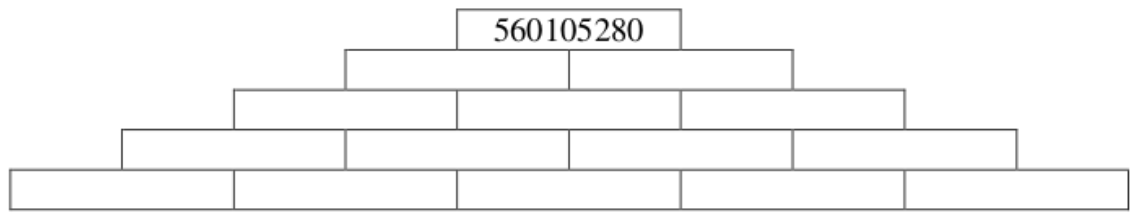
\includegraphics[scale=0.6]{Imagenes/IMG5/Piramide.png}
    \end{center}
\end{ejercicio}

\begin{ejercicio}
    Considere los reales positivos $p$ y $q$ tales que $p+q=1$. Demuestre que

    \begin{center}
        Si $r_k = \binom{n}{k} p^{k}q^{n-k}$, con $0 \leq k \leq n \ \Rightarrow \ \sum_{k=0}^{n} (k \cdot r_k) = np$
    \end{center}
\end{ejercicio}

\begin{ejercicio}
    Se construye un triángulo aritmético de la siguiente manera: primero se escriben en fila los números del 0 al 500, luego, cada número de la segunda fila es el resultado de sumar los dos números consecutivos de la primera fila que quedan justo sobre él y así se continúa formando el triángulo hasta que una de las filas está formada por solo un número. Demostrar que ese último número es múltiplo de 500.
\end{ejercicio}

\begin{ejercicio}
    Pruebe que el número de subconjuntos de $\{1, 2, ..., n\}$ con $k$ elementos y sin enteros consecutivos es

    \begin{center}
        $\binom{n+k+1}{k}$
    \end{center}
\end{ejercicio}

\begin{ejercicio}
    En la expansión $(\frac{20x^3}{y^5} + \frac{y^2}{x})^{67}$ determinar:

    \renewcommand{\labelenumi}{\alph{enumi})}
    \begin{enumerate}
        \item El vigésimo termino.
        \item El coeficiente del término cuarenta y cinco.
        \item El coeficiente de $x^{23}$, si es posible (si no, argumente por qué no existe).
        \item ¿Cuántos términos tiene la expansión?
    \end{enumerate}
\end{ejercicio}

\begin{ejercicio}
    Encuentre el coeficiente de $x^5$ en la expansión de $(1 +x+x^2)^8 + (1 +x+x^2)^9$.
\end{ejercicio}